% Provenance (never printed): see sources/outline_sources.md (Year 1: optical
% mineralogy with the polarising microscope; Michel-Levy chart). Interference
% colours in figdata/bachelor-1/michel_levy.py from the CIE 1931 colour-matching
% functions and illuminant D65 (data/derived/bachelor-1-cie*.csv); exercise and
% problem values in the Book 3 scratch calculator calc/ch08.py.
\chapter{光学矿物学}\label{ch:b1:optical-mineralogy}

在\omterm{def:b1:field-lab-methods-1:microscope}{正交偏光}下，一片辉长岩\omterm{def:b1:field-lab-methods-1:thin-section}{薄片}像彩色玻璃一样发光。
长条状的灰白色板条，纹理如条码，横贯视野；
板条之间，颗粒分别呈现蓝、黄和品红色，还有少数颗粒
无论转到哪个角度都保持黑色。这些现象各有可计算的成因，每一种都能说明其中是何种\omterm{def:b1:rock-forming-minerals:mineral}{矿物}。
本章讲解光如何穿过晶体，为何\omterm{def:b1:rock-forming-minerals:mineral}{矿物}在\omterm{def:b1:field-lab-methods-1:microscope}{正交偏光}下呈色，
颜色如何反映\omterm{def:b1:rock-forming-minerals:mineral}{矿物}的某种性质，以及岩石学家如何
仅凭一台显微镜命名\omterm{def:b1:field-lab-methods-1:thin-section}{薄片}中的颗粒。
本章最后分析一块未知\omterm{def:b1:field-lab-methods-1:thin-section}{薄片}，
由其呈现的现象求出其中的\omterm{def:b1:rock-forming-minerals:mineral}{矿物}及其真实厚度。

\begin{recall}
\omterm{def:b1:field-lab-methods-1:thin-section}{薄片}是厚约 \qty{30}{\micro m} 的岩石切片，
粘在玻璃载片上。\omterm{def:b1:field-lab-methods-1:microscope}{偏光显微镜}在\omterm{def:b1:field-lab-methods-1:microscope}{单偏光}（一个偏振片）下观察\omterm{def:b1:field-lab-methods-1:thin-section}{薄片}，
或在\omterm{def:b1:field-lab-methods-1:microscope}{正交偏光}下观察（见\cref{ch:b1:field-lab-methods-1}）。
介质的折射率 $n$ 为真空中的光速
与该介质中光速之比，光在界面处的折射遵循斯涅耳定律
$n_1\sin i_1 = n_2\sin i_2$（物理学，本科一年级）。光是横波；
偏振片只让电场中沿其方向的分量通过，
因此与之成 $\alpha$ 角的检偏器只让
强度的 $\cos^2\alpha$ 部分通过（马吕斯定律，物理学）。
\end{recall}

\section{晶体中的光}

在玻璃、液体或立方晶体中，光在各个方向上的传播速度相同，
与其振动方向无关。大多数\omterm{def:b1:rock-forming-minerals:mineral}{矿物}并非如此：
原子的排列沿不同方向各不相同，
电子对波电场的响应也随之不同。

\begin{definition}[均质矿物与非均质矿物]\label{def:b1:optical-mineralogy:anisotropic}
\omterm{def:b1:rock-forming-minerals:mineral}{矿物}的折射率对光的每一个传播方向和振动方向都相同时，称其为\emph{均质矿物}\index{均质矿物}；
立方晶系\omterm{def:b1:rock-forming-minerals:mineral}{矿物}（\omterm{def:b1:rock-forming-minerals:groups}{石榴子石}、岩盐、尖晶石）和玻璃都是均质的。
\omterm{def:b1:rock-forming-minerals:mineral}{矿物}的折射率随振动方向而变时，称其为
\emph{非均质矿物}\index{非均质矿物}；
其他晶系的\omterm{def:b1:rock-forming-minerals:mineral}{矿物}
都是非均质的。
\end{definition}

从非均质晶体切下的\omterm{def:b1:field-lab-methods-1:thin-section}{薄片}并不以单一
波的形式透光。我们承认晶体光学的如下结论（本科二年级物理学）：
对于给定的传播方向，\omterm{def:b1:optical-mineralogy:anisotropic}{非均质矿物}的\omterm{def:b1:field-lab-methods-1:thin-section}{薄片}
透过两束振动方向互相垂直、且固定于\omterm{def:b1:field-lab-methods-1:thin-section}{薄片}内的波，
称这两个方向为\emph{振动方向}，两束波以两个不同的折射率传播，
折射率分别为 $n_1$ 和 $n_2$。沿其中一个方向振动的光
穿过\omterm{def:b1:field-lab-methods-1:thin-section}{薄片}后偏振状态不变；沿任何其他方向振动的光
则被分解为沿这两个方向的两个分量。
两个折射率随传播方向而变，
并存在某些特定方向，使两者相等。

\begin{definition}[光轴，一轴晶与二轴晶]\label{def:b1:optical-mineralogy:optic-axis}
\omterm{def:b1:optical-mineralogy:anisotropic}{非均质矿物}的\emph{光轴}\index{光轴}是这样一个传播方向：
沿该方向传播的光只具有一个折射率，
与振动方向无关，与均质介质中的情形相同。\omterm{def:b1:rock-forming-minerals:mineral}{矿物}
只有一个光轴时，称为\emph{一轴晶}\index{一轴晶}（三方、四方和六方晶系的\omterm{def:b1:rock-forming-minerals:mineral}{矿物}，
如石英和方解石）；有两个光轴时，称为
\emph{二轴晶}\index{二轴晶}（斜方、单斜和三斜晶系的\omterm{def:b1:rock-forming-minerals:mineral}{矿物}，
如\omterm{def:b1:rock-forming-minerals:groups}{橄榄石}、\omterm{def:b1:rock-forming-minerals:groups}{辉石}、\omterm{def:b1:rock-forming-minerals:groups}{角闪石}、\omterm{def:b1:rock-forming-minerals:groups}{云母}和
\omterm{def:b1:rock-forming-minerals:groups}{长石}）。
\end{definition}

上述几何关系可用一个曲面概括，称为折射率椭球，它是这样一个椭球：
其在每一方向上的半径，即沿该方向振动的光的折射率。
与传播方向垂直的椭球截面是一个椭圆，
其两轴即两个振动方向，
其半轴长分别为 $n_1$ 和 $n_2$。对于\omterm{def:b1:optical-mineralogy:optic-axis}{一轴晶}，椭球
是绕\omterm{def:b1:optical-mineralogy:optic-axis}{光轴}的旋转椭球，有两个主折射率 $n_\omega$
和 $n_\varepsilon$：石英的 $n_\omega = 1.544$ 与 $n_\varepsilon = 1.553$，
方解石则为 $1.658$ 和 $1.486$。
% ledger: hom:quartz-optics, hom:calcite-optics
\omterm{def:b1:optical-mineralogy:optic-axis}{二轴晶}有三个主折射率 $n_\alpha < n_\beta < n_\gamma$，
并有两个圆截面，分别与其两个\omterm{def:b1:optical-mineralogy:optic-axis}{光轴}垂直。镁\omterm{def:b1:rock-forming-minerals:groups}{橄榄石}的
三个主折射率为 $1.635$、$1.651$ 和 $1.670$。
% ledger: hom:forsterite-optics

\begin{definition}[双折射率（矿物的）]\label{def:b1:optical-mineralogy:birefringence}
\omterm{def:b1:rock-forming-minerals:mineral}{矿物}的\emph{双折射率}\index{双折射率（矿物的）}为
其最大与最小主折射率之差 $\delta = n_{\max} - n_{\min}$：
\omterm{def:b1:optical-mineralogy:optic-axis}{一轴晶}取 $n_\varepsilon - n_\omega$ 的绝对值，
\omterm{def:b1:optical-mineralogy:optic-axis}{二轴晶}取 $n_\gamma - n_\alpha$。在
沿其他方向切割的颗粒中，差值 $|n_1 - n_2|$ 介于 0
（与\omterm{def:b1:optical-mineralogy:optic-axis}{光轴}垂直的截面）与 $\delta$（包含
$n_{\max}$ 与 $n_{\min}$ 方向的截面）之间。
\end{definition}

\omterm{def:b1:optical-mineralogy:birefringence}{双折射率}与密度一样，是\omterm{def:b1:rock-forming-minerals:mineral}{矿物}的一种性质：石英为
\num{0.009}，方解石为 \num{0.172}，镁\omterm{def:b1:rock-forming-minerals:groups}{橄榄石}为 \num{0.035}，铁\omterm{def:b1:rock-forming-minerals:groups}{橄榄石}
为 \num{0.052}。\omterm{def:b1:field-lab-methods-1:thin-section}{薄片}中同一种\omterm{def:b1:rock-forming-minerals:mineral}{矿物}的颗粒切割取向各不相同，
因此其颗粒呈现的数值从 0 到 $\delta$ 均有，只有
最高值才具有特征意义。
% ledger: hom:quartz-optics, hom:calcite-optics, hom:forsterite-optics, hom:fayalite-optics

\section{单偏光下的观察}

仅使用下偏振片时，显微镜可显示颗粒的形状、
颜色、解理和地形起伏。

\begin{definition}[多色性]\label{def:b1:optical-mineralogy:pleochroism}
\omterm{def:b1:rock-forming-minerals:mineral}{矿物}称为\emph{多色性的}\index{多色性}，当其在\omterm{def:b1:field-lab-methods-1:microscope}{单偏光}下
的颜色随载物台旋转而变化时；
这种变化即为\emph{多色性}。其成因是
光的吸收随其在晶体中的振动方向而不同。
\end{definition}

黑\omterm{def:b1:rock-forming-minerals:groups}{云母}是教科书中的典型例子：垂直于解理切出的颗粒在转动时由浅黄褐色
变为深褐色，解理迹线与起偏镜平行时颜色最深。
普通\omterm{def:b1:rock-forming-minerals:groups}{角闪石}由黄色变为绿色。其他多数
造岩硅酸盐（石英、\omterm{def:b1:rock-forming-minerals:groups}{长石}、\omterm{def:b1:rock-forming-minerals:groups}{橄榄石}、透\omterm{def:b1:rock-forming-minerals:groups}{辉石}、白\omterm{def:b1:rock-forming-minerals:groups}{云母}）在\omterm{def:b1:field-lab-methods-1:thin-section}{薄片}中
均为无色，其无色颗粒须
借助其他方法加以区分。
% ledger: hom:biotite-optics, hom:hornblende-optics, hom:muscovite-optics, hom:diopside-optics, hom:forsterite-optics

\begin{definition}[突起、贝克线]\label{def:b1:optical-mineralogy:relief}
\omterm{def:b1:field-lab-methods-1:thin-section}{薄片}中颗粒的\emph{突起}\index{突起（光学）}，是指其
轮廓、裂纹和表面相对于包埋介质的突出程度，
当颗粒与介质的折射率相差很大时突起高，
相近时则低。\emph{贝克线}\index{贝克线}是
折射率与周围物质不同的颗粒边缘所见的细亮线，
在显微镜略微离焦时可见。
\end{definition}

\begin{proposition}[突起与折射率]\label{prop:b1:optical-mineralogy:relief}
光线以入射角 $i$ 穿过折射率为 $n_m$ 的包埋介质与
折射率 $n$ 接近 $n_m$ 的颗粒之间的界面时，发生偏折，偏折角为
\[
  \varepsilon \approx \frac{|n - n_m|}{n_m}\,\tan i
\]
（以弧度计），且取 $(n - n_m)/n_m$ 的一阶近似。颗粒倾斜边缘处的偏折，
进而颗粒的\omterm{def:b1:optical-mineralogy:relief}{突起}，与
$|n - n_m|$ 成正比增大。
\end{proposition}

\begin{proof}
由斯涅耳定律得 $n_m \sin i = n \sin r$。记 $n = n_m(1 + \eta)$，其中
$\eta$ 为小量，$r = i - \varepsilon$，$\varepsilon$ 为小量。于是
$\sin i = (1 + \eta)(\sin i - \varepsilon\cos i) + O(\eta^2, \varepsilon^2)$,
故 $\eta \sin i = \varepsilon\cos i$，取一阶近似，即
$\varepsilon = \eta\tan i$，其中 $|\eta| = |n - n_m|/n_m$。
\end{proof}

\omterm{def:b1:field-lab-methods-1:thin-section}{薄片}包埋于折射率约为 $1.54$ 的树脂中。
% ledger: jaic:epoxy-ri
石英（$1.544$--$1.553$）与\omterm{def:b1:rock-forming-minerals:groups}{长石}（$1.52$--$1.59$）在其中几乎看不见，
\omterm{def:b1:optical-mineralogy:relief}{突起}低，颗粒边界难以分辨。\omterm{def:b1:rock-forming-minerals:groups}{橄榄石}
（$1.64$--$1.88$）、\omterm{def:b1:rock-forming-minerals:groups}{辉石}和\omterm{def:b1:rock-forming-minerals:groups}{角闪石}边缘发暗，表面看似粗糙，
\omterm{def:b1:optical-mineralogy:relief}{突起}高。\omterm{def:b1:rock-forming-minerals:groups}{石榴子石}（$1.83$）边缘几乎呈黑色。
方解石的折射率随振动方向在 $1.486$ 至 $1.658$ 之间变化，
转动载物台时其\omterm{def:b1:optical-mineralogy:relief}{突起}随之改变，这一效应称为“闪烁”。
% ledger: hom:quartz-optics, hom:albite-optics, hom:anorthite-optics, hom:orthoclase-optics, hom:forsterite-optics, hom:fayalite-optics, hom:almandine-optics, hom:calcite-optics
\omterm{def:b1:optical-mineralogy:relief}{突起}只说明 $n$ 与 $n_m$ 相差多少，不能说明偏向哪一侧；
偏向哪一侧则由\omterm{def:b1:optical-mineralogy:relief}{贝克线}判断。

\begin{method}[贝克线检验法]\label{met:b1:optical-mineralogy:becke}
在\omterm{def:b1:field-lab-methods-1:microscope}{单偏光}下将焦点对准颗粒边缘，略微缩小孔径光阑，
并稍稍提高焦点（使物镜远离\omterm{def:b1:field-lab-methods-1:thin-section}{薄片}）。
亮色的\omterm{def:b1:optical-mineralogy:relief}{贝克线}移向折射率较高的介质：
若移入颗粒，则颗粒折射率较高（正\omterm{def:b1:optical-mineralogy:relief}{突起}）；
若移出至包埋介质或相邻颗粒，
则颗粒折射率较低（负\omterm{def:b1:optical-mineralogy:relief}{突起}）。
\end{method}

此方法之所以有效，是因为颗粒边界从不完全竖直：在倾斜边界处，
光线向折射率较高的一侧偏折，
超过临界角时，光线在该侧发生全反射，于是穿过边界的光
集中在折射率较高的介质上方。
升高焦点即观察\omterm{def:b1:field-lab-methods-1:thin-section}{薄片}上方的一个平面，该处的汇聚光
正位于折射率较高的物质之中。

\section{正交偏光下}

插入与起偏镜成直角的检偏镜后，\omterm{def:b1:optical-mineralogy:anisotropic}{均质矿物}
颗粒在任何位置都呈黑色：光以沿起偏镜方向振动的方式射入，
又以同一方式射出，检偏镜将其完全挡住。
各向异性颗粒一般明亮且带有颜色，其原因
在于其两束波之间的延迟。

\begin{definition}[光程差（晶片中）]\label{def:b1:optical-mineralogy:retardation}
各向异性\omterm{def:b1:rock-forming-minerals:mineral}{矿物}晶片的\emph{光程差}\index{光程差（晶片中）} $\Delta$ 是
两束波离开晶片时的光程之差，
其中慢波滞后于快波。
\end{definition}

\begin{proposition}[光程差与双折射率]\label{prop:b1:optical-mineralogy:retardation}
厚度为 $d$、两束波折射率分别为 $n_1 > n_2$ 的晶片，其
\omterm{def:b1:optical-mineralogy:retardation}{光程差}为
\[
  \Delta = d\,(n_1 - n_2),
\]
两束波离开晶片时的相位差为 $\varphi = 2\pi\Delta/\lambda$
对真空中波长为 $\lambda$ 的光而言。在\omterm{def:b1:field-lab-methods-1:thin-section}{薄片}中，
同一\omterm{def:b1:rock-forming-minerals:mineral}{矿物}颗粒所显示的最大\omterm{def:b1:optical-mineralogy:retardation}{光程差}为 $d\,\delta$。
\end{proposition}

\begin{proof}
波穿过厚度为 $d$ 的晶片时，速度为 $c/n$，所需时间为 $nd/c$，其
光程即光在真空中该时间内所走的距离，为 $nd$。
两束波同时射入；射出时，慢波落后的光程为
$n_1 d - n_2 d = d(n_1 - n_2)$，这一延迟占 $\Delta/\lambda$ 个周期，
即相位 $2\pi\Delta/\lambda$。所有取向中
$n_1 - n_2$ 的最大值为 $\delta$
（见\cref{def:b1:optical-mineralogy:birefringence}）。
\end{proof}

\omterm{def:b1:field-lab-methods-1:thin-section}{薄片}中取向最有利的石英颗粒，
所在\omterm{def:b1:field-lab-methods-1:thin-section}{薄片}厚 \qty{30}{\micro m}，其 $\Delta = \qty{30000}{nm}\times0.009 =
\qty{270}{nm}$；方解石颗粒则为 $\qty{30000}{nm}\times0.172 = \qty{5160}{nm}$。

\begin{omfigure}
\begin{tikzpicture}[x=1cm, y=1cm, >={Stealth},
  sub/.style={align=center, font=\small, text width=4.2cm}]
% (a) the polariser
\begin{scope}
  \draw[gray!60] (-1.4,0) -- (1.4,0) (0,-1.4) -- (0,1.4);
  \node[gray, font=\scriptsize] at (1.55,-0.2) {东};
  \node[gray, font=\scriptsize] at (0.2,1.55) {北};
  \draw[very thick, omDef, <->] (-1.2,0) -- (1.2,0);
  \node[omDef, font=\scriptsize, above] at (0.75,0.05) {$E_0$};
  \node[sub] at (0,-2.1) {(a) 经起偏镜后：\\ 东西向振动};
\end{scope}
% (b) inside the plate
\begin{scope}[shift={(5.0,0)}]
  \draw[gray!60] (-1.4,0) -- (1.4,0) (0,-1.4) -- (0,1.4);
  \draw[omThm, thick] (-1.35*0.866,-1.35*0.5) -- (1.35*0.866,1.35*0.5);
  \draw[omThm, thick] (1.35*0.5,-1.35*0.866) -- (-1.35*0.5,1.35*0.866);
  \node[omThm, font=\scriptsize] at (1.42,0.95) {1};
  \node[omThm, font=\scriptsize] at (-0.85,1.32) {2};
  \draw[very thick, omDef, ->] (0,0) -- (1.2,0);
  \draw[omProp, very thick, ->] (0,0) -- (1.2*0.866*0.866,1.2*0.866*0.5);
  \draw[omProp, very thick, ->] (0,0) -- (1.2*0.5*0.5,-1.2*0.5*0.866);
  \draw[densely dotted] (1.2,0) -- (1.2*0.866*0.866,1.2*0.866*0.5) (1.2,0) -- (1.2*0.5*0.5,-1.2*0.5*0.866);
  \draw (0.55,0) arc[start angle=0, end angle=30, radius=0.55];
  \node[font=\scriptsize] at (0.75,0.17) {$\theta$};
  \node[omProp, font=\scriptsize] at (0.45,1.0) {$E_0\cos\theta$};
  \node[omProp, font=\scriptsize, anchor=east] at (0.1,-0.85) {$E_0\sin\theta$};
  \node[sub] at (0,-2.1) {(b) 晶片中：两束波分别沿 \\ 振动方向 1 和 2};
\end{scope}
% (c) at the analyser
\begin{scope}[shift={(10.0,0)}]
  \draw[gray!60] (-1.4,0) -- (1.4,0);
  \draw[very thick, omMeth, <->] (0,-1.3) -- (0,1.3);
  \node[omMeth, font=\scriptsize, right] at (0.05,1.2) {检偏镜};
  \draw[omProp, very thick, ->] (0,0) -- (1.2*0.866*0.866,1.2*0.866*0.5);
  \draw[omProp, very thick, ->] (0,0) -- (1.2*0.5*0.5,-1.2*0.5*0.866);
  \draw[densely dotted] (1.2*0.866*0.866,1.2*0.866*0.5) -- (0,1.2*0.866*0.5)
                        (1.2*0.5*0.5,-1.2*0.5*0.866) -- (0,-1.2*0.5*0.866);
  \draw[omMeth, very thick, ->] (0,0) -- (0,1.2*0.866*0.5);
  \draw[omMeth, very thick, ->] (0,0) -- (0,-1.2*0.5*0.866);
  \node[omMeth, font=\scriptsize, anchor=east] at (-0.08,0.52) {$+E_0\sin\theta\cos\theta$};
  \node[omMeth, font=\scriptsize, anchor=east] at (-0.08,-0.52) {$-E_0\sin\theta\cos\theta$};
  \node[sub] at (0,-2.1) {(c) 检偏镜处：每束波 \\ 通过其南北向分量};
\end{scope}
\end{tikzpicture}

{\small 光经过\omterm{def:b1:field-lab-methods-1:microscope}{正交偏光}之间的晶片。起偏镜
只让东西向振动通过（a）；晶片将其沿
自身振动方向分为两束波，它们与起偏镜的夹角分别为
$\theta$ 和 $\theta + \ang{90}$（b）；检偏镜为南北向，透过
每束波的南北向分量（c）。两个分量大小相等、符号相反：无延迟时
二者相互抵消，晶片呈暗色；波 2 落后于波 1 的
相位 $\varphi = 2\pi\Delta/\lambda$，两者之和不再为零。}
\end{omfigure}

\begin{theorem}[正交偏光之间的强度]\label{thm:b1:optical-mineralogy:intensity}
\omterm{def:b1:optical-mineralogy:retardation}{光程差}为 $\Delta$ 的晶片，其振动方向与起偏镜成
角 $\theta$，置于\omterm{def:b1:field-lab-methods-1:microscope}{正交偏光}之间，
在波长 $\lambda$ 处透过的强度为
\[
  I = I_0\,\sin^2 2\theta\,\sin^2\frac{\pi\Delta}{\lambda},
\]
其中 $I_0$ 为离开起偏镜的强度。
\end{theorem}

\begin{proof}
取起偏镜沿 $x$ 方向、检偏镜沿 $y$ 方向，
离开起偏镜的场为 $E_0 e^{i\omega t}$ 的实部（沿 $x$ 方向），
并取 $I_0 = E_0^2$（相差一个常数）。晶片的振动方向 1 为单位
矢量 $(\cos\theta, \sin\theta)$，方向 2 为 $(-\sin\theta, \cos\theta)$。
入射场沿方向 1 的分量为 $E_0\cos\theta$，
沿方向 2 的分量为 $-E_0\sin\theta$。晶片使波 1 保持不变（相差一个公共相位），
并使波 2 延迟 $\varphi = 2\pi\Delta/\lambda$
（\cref{prop:b1:optical-mineralogy:retardation}）；以复振幅表示，离开晶片的
波沿方向 1 为 $E_0\cos\theta$，
沿方向 2 为 $-E_0\sin\theta\,e^{-i\varphi}$。它们沿 $y$ 方向的分量分别为
$E_0\cos\theta\sin\theta$ 和 $-E_0\sin\theta\cos\theta\,e^{-i\varphi}$；
检偏镜透过二者之和，
\[
  A = E_0\sin\theta\cos\theta\,(1 - e^{-i\varphi}) .
\]
由于 $|1 - e^{-i\varphi}|^2 = 2 - 2\cos\varphi = 4\sin^2(\varphi/2)$ 且
$\sin\theta\cos\theta = \frac12\sin2\theta$，故强度为
$|A|^2 = E_0^2\,\sin^2 2\theta\,\sin^2(\varphi/2)$，即
$I = I_0\sin^2 2\theta\sin^2(\pi\Delta/\lambda)$。若波 1 为慢波，
则 $\varphi$ 变号，$I$ 保持不变。
\end{proof}

该定理包含了显微镜在\omterm{def:b1:field-lab-methods-1:microscope}{正交偏光}之间所呈现的全部内容。第一个因子
只取决于颗粒在载物台上的方位，
第二个因子只取决于颗粒的\omterm{def:b1:optical-mineralogy:retardation}{光程差}
以及光的颜色。

\begin{definition}[消光位、消光角]\label{def:b1:optical-mineralogy:extinction}
在\omterm{def:b1:field-lab-methods-1:microscope}{正交偏光}之间，非均质颗粒处于\emph{消光位}\index{消光位}
时，因其振动方向与起偏镜和检偏镜平行而呈暗色。
颗粒的
\emph{消光角}\index{消光角}是指颗粒中某一可见方向
（解理迹、伸长方向或\omterm{def:b1:optical-mineralogy:twin}{双晶}面）与最近的消光位
之间的夹角，在刻度载物台上读出。
\end{definition}

因子 $\sin^2 2\theta$ 在 $\theta = 0$、\ang{90}、\ang{180} 和
\ang{270} 处为零：颗粒在载物台转动一周内四次变暗，
并在两\omterm{def:b1:optical-mineralogy:extinction}{消光位}中间、距\omterm{def:b1:optical-mineralogy:extinction}{消光位} \ang{45} 处最亮（见下图）。
\omterm{def:b1:optical-mineralogy:retardation}{光程差} $\Delta = 0$ 的颗粒——即\omterm{def:b1:optical-mineralogy:anisotropic}{均质矿物}，或垂直于\omterm{def:b1:optical-mineralogy:optic-axis}{光轴}的
切面——始终保持暗色。\omterm{def:b1:optical-mineralogy:extinction}{消光角}取决于晶体的对称性：
振动方向与解理相关的\omterm{def:b1:rock-forming-minerals:mineral}{矿物}，如斜方晶系\omterm{def:b1:rock-forming-minerals:mineral}{矿物}，
平行于解理消光（平行消光）；
单斜或三斜晶系\omterm{def:b1:rock-forming-minerals:mineral}{矿物}一般不然（斜消光）。
解理迹与慢振动方向之间的最大\omterm{def:b1:optical-mineralogy:extinction}{消光角}
在透\omterm{def:b1:rock-forming-minerals:groups}{辉石}中约为 \ang{38}，在普通\omterm{def:b1:rock-forming-minerals:groups}{角闪石}中为
\ang{15}--\ang{19}，切面平行于 $(010)$，
这是在\omterm{def:b1:field-lab-methods-1:thin-section}{薄片}中区分\omterm{def:b1:rock-forming-minerals:groups}{辉石}与\omterm{def:b1:rock-forming-minerals:groups}{角闪石}的方法之一。
% ledger: hom:diopside-optics, hom:hornblende-optics

\begin{omfigure}
\begin{tikzpicture}
\begin{axis}[width=0.8\linewidth, height=5cm, xmin=0, xmax=360, ymin=0, ymax=1.08,
  xtick={0,45,90,...,360}, ytick={0,0.5,1},
  tick label style={font=\scriptsize}, label style={font=\small},
  xlabel={距消光位的载物台角 $\theta$（\si{\degree}）},
  ylabel={$I/I_0$}, legend style={font=\scriptsize, at={(0.5,1.03)}, anchor=south, legend columns=3,
  draw=none}, legend cell align=left]
\addplot[omThm, thick] table[x=theta, y=I270] {figdata/out/bachelor-1-michel_levy-rotation.dat};
\addplot[omDef, thick, densely dashed] table[x=theta, y=I100] {figdata/out/bachelor-1-michel_levy-rotation.dat};
\addplot[omMeth, thick, densely dotted] table[x=theta, y=I540] {figdata/out/bachelor-1-michel_levy-rotation.dat};
\legend{$\Delta = \qty{270}{nm}$, $\Delta = \qty{100}{nm}$, $\Delta = \qty{540}{nm}$}
\end{axis}
\end{tikzpicture}

{\small 颗粒随载物台转动时透过的强度，波长为
\qty{550}{nm}，三种\omterm{def:b1:optical-mineralogy:retardation}{光程差}下的结果（\cref{thm:b1:optical-mineralogy:intensity}）。
每转一周四次消光、四次极大，极大出现在距\omterm{def:b1:optical-mineralogy:extinction}{消光位} \ang{45} 处；
\omterm{def:b1:optical-mineralogy:retardation}{光程差}决定极大值的高度，当 $\Delta$ 接近
波长的整数倍时，极大值几乎为零。}
\end{omfigure}

\subsection{干涉色}

在白光下，第二个因子 $\sin^2(\pi\Delta/\lambda)$ 起着
随波长变化的滤光作用。\omterm{def:b1:optical-mineralogy:retardation}{光程差} $\Delta = \qty{270}{nm}$ 的颗粒
几乎透过全部绿光和黄光（$\lambda$ 接近 $2\Delta = 540$\,nm，
此时因子为 1），对紫光和红光的透过略少：
呈白色。\omterm{def:b1:optical-mineralogy:retardation}{光程差} $\Delta = \qty{550}{nm}$ 的颗粒抑制黄绿光
（$\lambda = \Delta$），透过红光和蓝光：呈品红色。随着 $\Delta$
增大，被抑制的波长在光谱中移动，
又不断出现新的被抑制波长，颜色按固定顺序变化。

\begin{definition}[干涉色、级次、米歇尔–莱维色谱表]\label{def:b1:optical-mineralogy:interference-colour}
非均质颗粒的\emph{干涉色}\index{干涉色}是
它在白光下、\omterm{def:b1:field-lab-methods-1:microscope}{正交偏光}之间、距\omterm{def:b1:optical-mineralogy:extinction}{消光位} \ang{45} 处的颜色，
仅取决于其\omterm{def:b1:optical-mineralogy:retardation}{光程差} $\Delta$。颜色按约
\qty{550}{nm} 的\omterm{def:b1:optical-mineralogy:retardation}{光程差}为周期重复出现，每个周期以红紫色调结束；
每个周期即一个\emph{级次}\index{级次（干涉色）}
（第一、第二、第三\dots）。\emph{米歇尔–莱维
色谱表}\index{米歇尔–莱维色谱表}给出干涉色随
\omterm{def:b1:optical-mineralogy:retardation}{光程差}的变化，图中各线 $\Delta = d\,\delta$ 表示
\omterm{def:b1:field-lab-methods-1:thin-section}{薄片}厚度、\omterm{def:b1:rock-forming-minerals:mineral}{矿物}\omterm{def:b1:optical-mineralogy:birefringence}{双折射率}与其颜色之间的关系。
\end{definition}

\begin{omfigure}
\begin{tikzpicture}
\begin{axis}[width=0.84\linewidth, height=7.2cm, view={0}{90}, xmin=0, xmax=1800, ymin=0, ymax=50,
  xtick={0,200,...,1800}, ytick={0,10,...,50}, axis on top, clip=false,
  tick label style={font=\scriptsize}, label style={font=\small},
  xlabel={光程差 $\Delta$ (nm)}, ylabel={厚度 $d$ (\si{\micro m})},
  unbounded coords=jump]
\addplot3[surf, shader=flat corner, mesh/cols=361, mesh/color input=explicit mathparse,
  point meta={symbolic={\thisrow{r},\thisrow{g},\thisrow{b}}}]
  table[x=delta, y=d, z expr=0] {figdata/out/bachelor-1-michel_levy-chart.dat};
\addplot3[black, thin] table[x=x, y=y, z expr=0] {figdata/out/bachelor-1-michel_levy-segments.dat};
\addplot3[white, very thick, densely dashed] coordinates {(0,30,0) (1800,30,0)};
\node[font=\tiny, anchor=south west, rotate=60] at (axis cs:250,50.3,0) {正长石 0.005};
\node[font=\tiny, anchor=south west, rotate=60] at (axis cs:450,50.3,0) {石英 0.009};
\node[font=\tiny, anchor=south west, rotate=60] at (axis cs:600,50.3,0) {斜长石 0.012};
\node[font=\tiny, anchor=south west, rotate=60] at (axis cs:1000,50.3,0) {普通角闪石 0.020};
\node[font=\tiny, anchor=south west, rotate=60] at (axis cs:1500,50.3,0) {透辉石 0.030};
\node[font=\tiny, anchor=south west, rotate=60] at (axis cs:1750,50.3,0) {镁橄榄石 0.035};
\node[font=\tiny, anchor=west] at (axis cs:1810,45,0) {白云母 0.040};
\node[font=\tiny, anchor=west] at (axis cs:1810,34.6,0) {铁橄榄石 0.052};
\node[font=\tiny, anchor=west] at (axis cs:1810,10.5,0) {方解石 0.172};
\node[font=\tiny, anchor=west] at (axis cs:1810,30,0) {\qty{30}{\micro m}};
\node[font=\scriptsize, anchor=north] at (axis cs:270,-7,0) {一级};
\node[font=\scriptsize, anchor=north] at (axis cs:808,-7,0) {二级};
\node[font=\scriptsize, anchor=north] at (axis cs:1340,-7,0) {三级};
\end{axis}
\end{tikzpicture}

{\small 由第一性原理计算的\omterm{def:b1:optical-mineralogy:interference-colour}{米歇尔–莱维色谱表}：对每个\omterm{def:b1:optical-mineralogy:retardation}{光程差}，
白光（CIE 标准光源 D65）经\omterm{def:b1:field-lab-methods-1:microscope}{正交偏光}及距\omterm{def:b1:optical-mineralogy:extinction}{消光位} \ang{45} 处的\omterm{def:b1:field-lab-methods-1:thin-section}{薄片}后所呈的颜色，
依据 CIE 1931 色度匹配函数
（数据 \textcopyright{} CIE，CC BY-SA 4.0）及 sRGB 变换算得，
并以平行偏光透过的光强归一化。黑线给出各\omterm{def:b1:rock-forming-minerals:mineral}{矿物}
\omterm{def:b1:optical-mineralogy:birefringence}{双折射率}对应的 $\Delta = d\,\delta$；虚线为标准厚度 \qty{30}{\micro m}。
各\omterm{def:b1:optical-mineralogy:interference-colour}{级次}末端的红紫色调
在本计算中落于 542、1074 和 \qty{1605}{nm}
处。}
% ledger: data:b3-cie1931, data:b3-cie-d65, w3c:srgb, hom:orthoclase-optics, hom:quartz-optics, hom:albite-optics, hom:anorthite-optics, hom:hornblende-optics, hom:diopside-optics, hom:forsterite-optics, hom:muscovite-optics, hom:fayalite-optics, hom:calcite-optics
\end{omfigure}

色谱表严格按定理所述计算。对每个\omterm{def:b1:optical-mineralogy:retardation}{光程差}，
光的每个波长以 $\sin^2(\pi\Delta/\lambda)$ 加权；
透过的光谱再依人眼所见转化为颜色，
采用比色学中的标准色度匹配函数，
再经 sRGB 变换得到屏幕或打印机所用的红、绿、蓝分量。值得注意的有三点。
第一\omterm{def:b1:optical-mineralogy:interference-colour}{级次}由黑色起，经灰色和白色，
（色谱中唯一的白色位于 \qty{270}{nm} 附近，此处光谱几乎全部透过），
再呈黄色、橙色和红色。
第二、第三\omterm{def:b1:optical-mineralogy:interference-colour}{级次}最为鲜亮，呈现鲜艳的蓝、绿、黄和品红。
越过第四\omterm{def:b1:optical-mineralogy:interference-colour}{级次}后颜色渐淡：当 $\Delta$ 为许多个波长时，
滤波器 $\sin^2(\pi\Delta/\lambda)$ 在可见光谱内振荡数次，
依次透过每种颜色，平均而言仅透过约一半的光，
颗粒呈淡粉色或灰绿色，
即方解石的高级白色。

读图是光性\omterm{def:b1:rock-forming-minerals:mineral}{矿物}学的核心。在厚度已知的\omterm{def:b1:field-lab-methods-1:thin-section}{薄片}中，
\omterm{def:b1:rock-forming-minerals:mineral}{矿物}所呈现的最高\omterm{def:b1:optical-mineralogy:interference-colour}{干涉色}给出其\omterm{def:b1:optical-mineralogy:birefringence}{双折射率}：
从厚度处横向找到该颜色，再沿过该点的线
读出其\omterm{def:b1:optical-mineralogy:birefringence}{双折射率}。反之，已知\omterm{def:b1:optical-mineralogy:birefringence}{双折射率}的\omterm{def:b1:rock-forming-minerals:mineral}{矿物}给出厚度：
在良好的 \qty{30}{\micro m} \omterm{def:b1:field-lab-methods-1:thin-section}{薄片}中，石英
至多只呈一级白色或极淡的黄色，
若石英呈现黄色或橙色，则\omterm{def:b1:field-lab-methods-1:thin-section}{薄片}过厚。

\begin{history}[奥古斯特·米歇尔–莱维]
% ledger: annales:michel-levy, annales:michel-levy-director, commons:michel-levy
\begin{minipage}[t]{0.76\linewidth}\vspace{0pt}
奥古斯特·米歇尔–莱维（1844--1911）曾任法国地质调查局局长，
是最早系统借助\omterm{def:b1:field-lab-methods-1:microscope}{偏光显微镜}鉴定岩石中\omterm{def:b1:rock-forming-minerals:mineral}{矿物}的学者之一。
在他之前，\omterm{def:b1:rock-forming-minerals:mineral}{矿物}在\omterm{def:b1:field-lab-methods-1:microscope}{正交偏光}下的颜色仅被经验地使用；
他指出，关键在于各\omterm{def:b1:rock-forming-minerals:mineral}{矿物}的最大\omterm{def:b1:optical-mineralogy:birefringence}{双折射率}，
它可通过将其颗粒的颜色与一块\omterm{def:b1:optical-mineralogy:retardation}{光程差}沿长度稳定增加的
石英楔相比对而测得。
他与学生阿尔弗雷德·拉克卢瓦于 1888 年
合著出版 \emph{Les minéraux des roches}，这是一部关于造岩\omterm{def:b1:rock-forming-minerals:mineral}{矿物}光学性质的手册。
以他命名的色谱表以颜色对\omterm{def:b1:optical-mineralogy:retardation}{光程差}作图，
并附有等\omterm{def:b1:optical-mineralogy:birefringence}{双折射率}线，
至今仍是读取\omterm{def:b1:optical-mineralogy:interference-colour}{干涉色}的通用方法。
\end{minipage}\hfill
\begin{minipage}[t]{0.2\linewidth}\vspace{0pt}
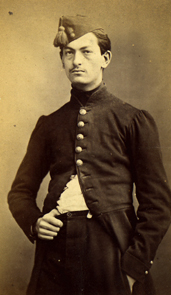
\includegraphics[width=\linewidth]{images/book3/b1-michel-levy.jpg}

{\scriptsize 米歇尔–莱维学生时期，约 1862 年。公有领域。}
\end{minipage}
\end{history}

从颗粒射出的两束波，可借助插入在\omterm{def:b1:field-lab-methods-1:thin-section}{薄片}上方的试板
（与偏光镜成 \ang{45} 角）获得一个已知的附加\omterm{def:b1:optical-mineralogy:retardation}{光程差}。
最常用的一种试板切成可显示一级红色的形式，\omterm{def:b1:optical-mineralogy:retardation}{光程差}约为 \qty{540}{nm}。
若颗粒的慢振动方向与试板的慢方向平行，则\omterm{def:b1:optical-mineralogy:retardation}{光程差}相加，
颗粒的颜色升高约一个\omterm{def:b1:optical-mineralogy:interference-colour}{级次}；
若与快方向平行，则相减，颜色降低。
一个一级灰色的颗粒，\omterm{def:b1:optical-mineralogy:retardation}{光程差}为 \qty{100}{nm}，
在一种取向下变为二级蓝色（\qty{640}{nm}），
在另一种取向下变为一级橙色（\qty{440}{nm}）；
由此可判定颗粒两个振动方向中哪一个为慢方向，
这一性质可用于鉴定拉长状\omterm{def:b1:rock-forming-minerals:mineral}{矿物}。

\section{在薄片中鉴定矿物}

\begin{definition}[双晶、聚片双晶]\label{def:b1:optical-mineralogy:twin}
称\emph{双晶}\index{双晶}为同种\omterm{def:b1:rock-forming-minerals:mineral}{矿物}的两个或多个晶体的连生，
其晶格之间存在晶体本身不具有的对称关系，
例如关于某一平面（双晶面）的反映。
\emph{聚片双晶}\index{聚片双晶}是沿平行面的重复双晶，
使晶体分割为相互平行的片晶，
各片晶的取向相互交替。
\end{definition}

在\omterm{def:b1:field-lab-methods-1:microscope}{正交偏光}下，\omterm{def:b1:optical-mineralogy:twin}{聚片双晶}的各片晶交替消光：
一半片晶暗时另一半恰好亮，晶体呈现条纹状。
\omterm{def:b1:rock-forming-minerals:groups}{斜长石}几乎总是呈现这种条纹，
据此可将其与石英及\omterm{def:b1:rock-forming-minerals:groups}{碱性长石}立即区分；
其另一特征，即低\omterm{def:b1:optical-mineralogy:relief}{突起}和一级灰至白的\omterm{def:b1:optical-mineralogy:interference-colour}{干涉色}，与它们相同。
\omterm{def:b1:optical-mineralogy:twin}{双晶}面两侧所测得的两组片晶\omterm{def:b1:optical-mineralogy:extinction}{消光角}
取决于\omterm{def:b1:rock-forming-minerals:groups}{斜长石}的成分，
由这些角度的图表可求得其钙\omterm{def:b1:rock-forming-minerals:groups}{长石}含量。

\begin{method}[薄片中矿物的鉴定]\label{met:b1:optical-mineralogy:identify}
\begin{enumerate}
  \item 在\omterm{def:b1:field-lab-methods-1:microscope}{单偏光}下：观察颗粒是否不透明；其
        颜色和\omterm{def:b1:optical-mineralogy:pleochroism}{多色性}（转动载物台）；其\omterm{def:b1:optical-mineralogy:relief}{突起}，以及其折射率位于
        $1.54$ 的哪一侧（\omterm{def:b1:optical-mineralogy:relief}{贝克线}）；其形状和解理，
        以及两组解理之间的夹角。
  \item 在\omterm{def:b1:field-lab-methods-1:microscope}{正交偏光}下：检查其是否保持暗色（均质体，或
        垂直于\omterm{def:b1:optical-mineralogy:optic-axis}{光轴}的切面）；在同种\omterm{def:b1:rock-forming-minerals:mineral}{矿物}的颗粒中，
        找出最高\omterm{def:b1:optical-mineralogy:interference-colour}{干涉色}，并
        依据\omterm{def:b1:field-lab-methods-1:thin-section}{薄片}厚度，
        在米歇尔–列维色谱表上读出\omterm{def:b1:optical-mineralogy:birefringence}{双折射率}。
  \item 在显示解理或延长方向的颗粒上测量\omterm{def:b1:optical-mineralogy:extinction}{消光角}；
        观察是否存在\omterm{def:b1:optical-mineralogy:twin}{双晶}（聚片条纹、简单\omterm{def:b1:optical-mineralogy:twin}{双晶}）。
  \item 与光学性质表
        （\cref{tab:b1:optical-mineralogy:key}）及岩石中可能含有的
        \omterm{def:b1:rock-forming-minerals:mineral}{矿物}（\cref{ch:b1:rock-forming-minerals}）相比较。
\end{enumerate}
\end{method}

\begin{table}[htbp]
\centering\footnotesize
\setlength{\tabcolsep}{3pt}
% ledger: hom:quartz-optics, hom:orthoclase-optics, hom:albite-optics, hom:anorthite-optics, hom:muscovite-optics, hom:biotite-optics, hom:hornblende-optics, hom:diopside-optics, hom:forsterite-optics, hom:fayalite-optics, hom:almandine-optics, hom:calcite-optics, hom:magnetite-optics
\begin{tabular}{@{}>{\raggedright\arraybackslash}p{2.0cm}>{\raggedright\arraybackslash}p{2.6cm}>{\raggedright\arraybackslash}p{2.3cm}>{\raggedright\arraybackslash}p{1.8cm}>{\raggedright\arraybackslash}p{3.0cm}>{\raggedright\arraybackslash}p{3.8cm}@{}}
\hline
\omterm{def:b1:rock-forming-minerals:mineral}{矿物} & 颜色（\omterm{def:b1:field-lab-methods-1:microscope}{单偏光}） & 折射率 & \omterm{def:b1:optical-mineralogy:birefringence}{双折射率} & 厚 \qty{30}{\micro m} 时的最高\omterm{def:b1:optical-mineralogy:interference-colour}{干涉色} & 其他特征 \\
\hline
石英 & 无色 & 1.544--1.553 & 0.009 & 一级白 & 无解理；不见\omterm{def:b1:optical-mineralogy:twin}{双晶}；\omterm{def:b1:optical-mineralogy:optic-axis}{一轴晶} \\
正\omterm{def:b1:rock-forming-minerals:groups}{长石} & 无色，常浑浊 & 1.518--1.525 & 0.005 & 一级灰 & 负\omterm{def:b1:optical-mineralogy:relief}{突起}；简单\omterm{def:b1:optical-mineralogy:twin}{双晶} \\
\omterm{def:b1:rock-forming-minerals:groups}{斜长石} & 无色 & 1.526--1.590 & 0.008--0.013 & 一级白至淡黄 & \omterm{def:b1:optical-mineralogy:twin}{聚片双晶} \\
白\omterm{def:b1:rock-forming-minerals:groups}{云母} & 无色 & 1.552--1.618 & 0.035--0.042 & 鲜艳的二级至三级 & 一组完全解理；平行消光 \\
黑\omterm{def:b1:rock-forming-minerals:groups}{云母} & 褐色、绿色 & 1.565--1.696 & 0.04--0.07 & 被自身颜色掩盖 & 强\omterm{def:b1:optical-mineralogy:pleochroism}{多色性}；一组完全解理 \\
\omterm{def:b1:rock-forming-minerals:groups}{角闪石} & 绿色、褐色 & 1.675--1.695 & 0.020 & 二级蓝 & \omterm{def:b1:optical-mineralogy:pleochroism}{多色性}；解理夹角 \ang{56}/\ang{124}；\omterm{def:b1:optical-mineralogy:extinction}{消光角} \ang{15}--\ang{19} \\
透\omterm{def:b1:rock-forming-minerals:groups}{辉石} & 无色 & 1.664--1.694 & 0.030 & 二级黄 & 解理夹角约 \ang{87}/\ang{93}；\omterm{def:b1:optical-mineralogy:extinction}{消光角}约 \ang{38} \\
\omterm{def:b1:rock-forming-minerals:groups}{橄榄石} & 无色（镁质）至淡黄（铁质） & 1.635--1.879 & 0.035--0.052 & 二级末至三级 & 高\omterm{def:b1:optical-mineralogy:relief}{突起}；不规则裂隙，无良好解理 \\
\omterm{def:b1:rock-forming-minerals:groups}{石榴子石} & 无色至淡粉红 & 1.830（铁铝榴石） & 均质 & 黑 & 极高\omterm{def:b1:optical-mineralogy:relief}{突起}；六边形或八边形轮廓 \\
方解石 & 无色 & 1.486--1.658 & 0.172 & 高级白 & 转动时\omterm{def:b1:optical-mineralogy:relief}{突起}变化；菱面体解理 \\
磁铁矿 & 不透明 &——&——&——& 两种光下均为黑色 \\
\hline
\end{tabular}
\caption{\omterm{def:b1:field-lab-methods-1:thin-section}{薄片}中常见造岩\omterm{def:b1:rock-forming-minerals:mineral}{矿物}的光学性质。
\omterm{def:b1:field-lab-methods-1:microscope}{单偏光}：PPL。最高\omterm{def:b1:optical-mineralogy:interference-colour}{干涉色}在米歇尔–列维
色谱表上按 $\Delta = \qty{30000}{nm}\times\delta$ 读出。}
\label{tab:b1:optical-mineralogy:key}
\end{table}

\begin{omfigure}
\setlength{\tabcolsep}{2pt}
\begin{tabular}{cc}
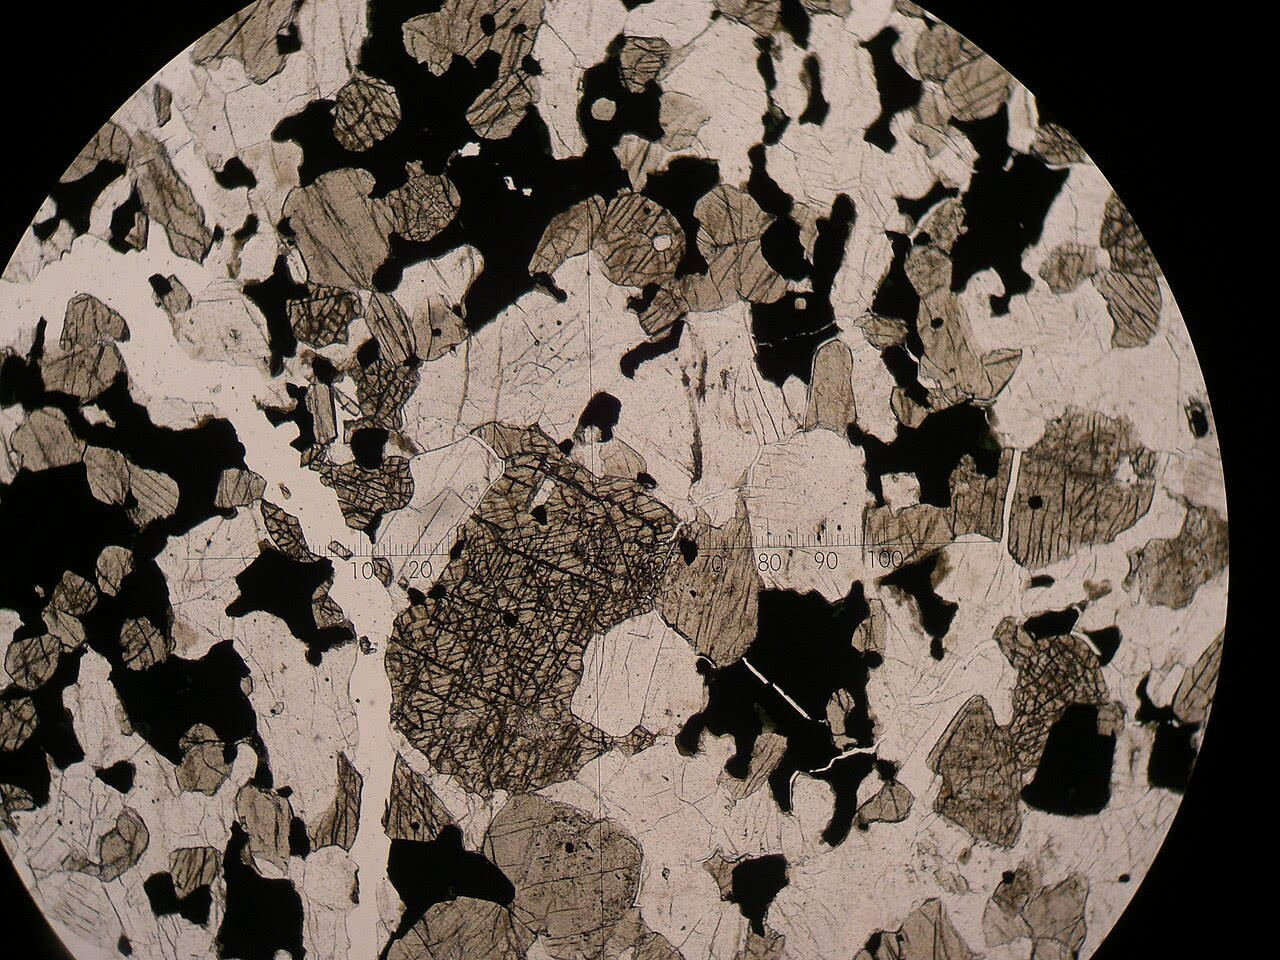
\includegraphics[width=0.485\linewidth]{images/book3/b1-gabbro-ppl.jpg} &
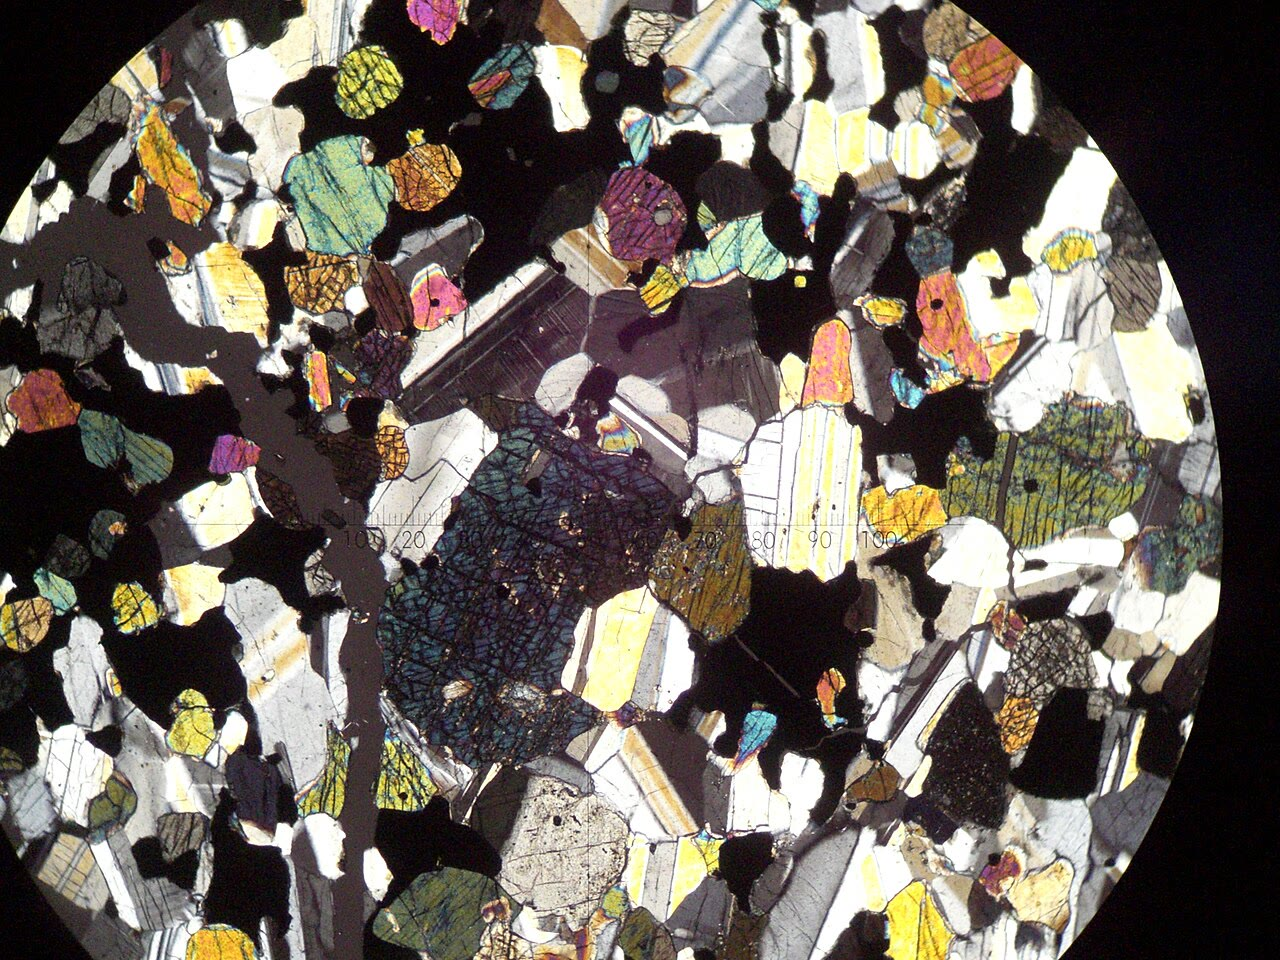
\includegraphics[width=0.485\linewidth]{images/book3/b1-gabbro-xpl.jpg} \\
{\small （a）\omterm{def:b1:field-lab-methods-1:microscope}{单偏光}} & {\small （b）\omterm{def:b1:field-lab-methods-1:microscope}{正交偏光}} \\
\end{tabular}
% ledger: commons:gabbro-ppl, commons:gabbro-xpl

\medskip
{\small 同一视域下辉长岩的\omterm{def:b1:field-lab-methods-1:thin-section}{薄片}。\omterm{def:b1:field-lab-methods-1:microscope}{单偏光}
（a）下，\omterm{def:b1:rock-forming-minerals:groups}{斜长石}无色、\omterm{def:b1:optical-mineralogy:relief}{突起}低；\omterm{def:b1:rock-forming-minerals:groups}{辉石}和\omterm{def:b1:rock-forming-minerals:groups}{橄榄石}
颗粒呈浅褐灰色，\omterm{def:b1:optical-mineralogy:relief}{突起}高，裂隙密集；不透明的
矿石为黑色；目镜中的标尺为一微米。\omterm{def:b1:field-lab-methods-1:microscope}{正交偏光}
（b）下，\omterm{def:b1:rock-forming-minerals:groups}{斜长石}条带因\omterm{def:b1:optical-mineralogy:twin}{聚片双晶}而呈条纹状，
\omterm{def:b1:rock-forming-minerals:groups}{辉石}和\omterm{def:b1:rock-forming-minerals:groups}{橄榄石}颗粒呈二级\omterm{def:b1:optical-mineralogy:interference-colour}{干涉色}，矿石仍为
黑色。照片：Chmee2，CC BY-SA 3.0（维基共享资源）。}
\end{omfigure}

\begin{inthelab}[在显微镜下的一次观察]
\begin{minipage}[t]{0.55\linewidth}\vspace{0pt}
岩石学家描述一块新的\omterm{def:b1:field-lab-methods-1:thin-section}{薄片}时，先在低倍下
观察其结构和主要\omterm{def:b1:rock-forming-minerals:mineral}{矿物}，再逐颗粒进行研究。
对每种\omterm{def:b1:rock-forming-minerals:mineral}{矿物}，她记录上述方法所得的观察结果，
估计其在视域中所占的比例，并注意颗粒间的接触关系：
哪种先结晶，哪种充填剩余的空隙，哪种交代其他\omterm{def:b1:rock-forming-minerals:mineral}{矿物}。
光学测量时使用带刻度的载物台和附加补偿器；
需要时，成分将在之后用电子探针在同一\omterm{def:b1:field-lab-methods-1:thin-section}{薄片}上测定。
教学实验室的做法与此相同，
每名学生一台显微镜，旁边放一盒已知\omterm{def:b1:rock-forming-minerals:mineral}{矿物}的参考\omterm{def:b1:field-lab-methods-1:thin-section}{薄片}。
\end{minipage}\hfill
\begin{minipage}[t]{0.42\linewidth}\vspace{0pt}
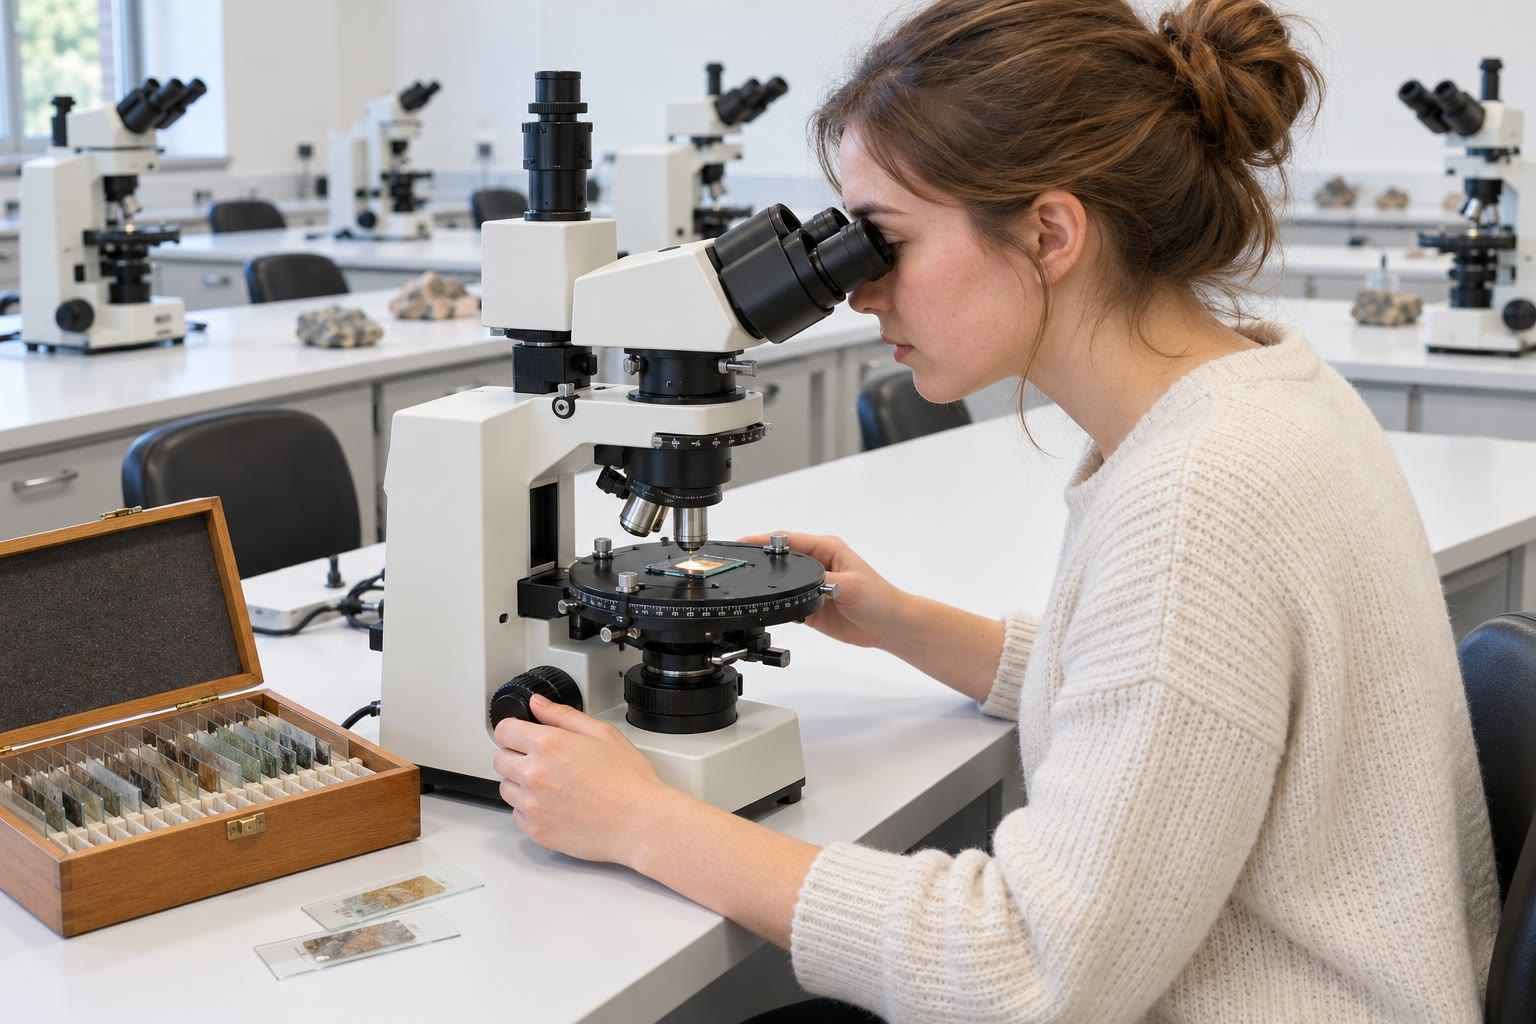
\includegraphics[width=\linewidth]{images/book3/ai/b1-microscope-student.jpg}

{\scriptsize 教学实验室中，一名学生正在使用\omterm{def:b1:field-lab-methods-1:microscope}{偏光显微镜}
（AI 生成的插图）。}
\end{minipage}
\end{inthelab}

\section{练习}

\begin{exercise}[$\star$]\label{exo:b1:optical-mineralogy:1}
计算石英（$\delta = 0.009$）与方解石
（$\delta = 0.172$）在厚 \qty{30}{\micro m} 的\omterm{def:b1:field-lab-methods-1:thin-section}{薄片}中的最大\omterm{def:b1:optical-mineralogy:retardation}{光程差}。利用
米歇尔–列维色谱表，描述二者各自的颜色。
% ledger: hom:quartz-optics, hom:calcite-optics
\end{exercise}

\begin{exercise}[$\star$]\label{exo:b1:optical-mineralogy:2}
在\omterm{def:b1:field-lab-methods-1:microscope}{正交偏光}下转动载物台上的某一颗粒。计算 $I/I_0$（以其最大值的分数表示），
在距\omterm{def:b1:optical-mineralogy:extinction}{消光位}的夹角 $\theta = 0$、\ang{22.5}、\ang{45}、\ang{67.5} 和
\ang{90} 处各值。
\end{exercise}

\begin{exercise}[$\star$]\label{exo:b1:optical-mineralogy:3}
解释为何\omterm{def:b1:rock-forming-minerals:groups}{石榴子石}在\omterm{def:b1:field-lab-methods-1:microscope}{正交偏光}下，无论载物台处于何种位置，都保持黑色，
以及石英颗粒为何也可能如此。在\omterm{def:b1:field-lab-methods-1:microscope}{单偏光}下，
你将如何区分二者？
\end{exercise}

\begin{exercise}[$\star$]\label{exo:b1:optical-mineralogy:4}
在折射率为 $1.54$ 的封固介质中，按\omterm{def:b1:optical-mineralogy:relief}{突起}大小将下列\omterm{def:b1:rock-forming-minerals:mineral}{矿物}排序：正\omterm{def:b1:rock-forming-minerals:groups}{长石}（$n$ 约 $1.52$），
石英（$1.55$）、镁\omterm{def:b1:rock-forming-minerals:groups}{橄榄石}（$1.65$）和铁铝榴石（$1.83$）。哪一种
具有负\omterm{def:b1:optical-mineralogy:relief}{突起}？其\omterm{def:b1:optical-mineralogy:relief}{贝克线}在升高焦点时
向哪个方向移动？
% ledger: hom:orthoclase-optics, hom:quartz-optics, hom:forsterite-optics, hom:almandine-optics
\end{exercise}

\begin{exercise}[$\star\star$]\label{exo:b1:optical-mineralogy:5}
在 \qty{30}{\micro m} 厚的\omterm{def:b1:field-lab-methods-1:thin-section}{薄片}中，一种绿色\omterm{def:b1:optical-mineralogy:pleochroism}{多色性}\omterm{def:b1:rock-forming-minerals:mineral}{矿物}的颗粒
具有两组解理，夹角分别为 \ang{56} 和 \ang{124}，至多呈二级蓝色，
在色谱表上读得 $\Delta = \qty{650}{nm}$。计算其\omterm{def:b1:optical-mineralogy:birefringence}{双折射率}，并
借助\cref{tab:b1:optical-mineralogy:key}确定该\omterm{def:b1:rock-forming-minerals:mineral}{矿物}的名称。
\end{exercise}

\begin{exercise}[$\star\star$]\label{exo:b1:optical-mineralogy:6}
利用\cref{prop:b1:optical-mineralogy:relief}，取 $n_m = 1.54$ 和
$i = \ang{30}$，计算石英颗粒（$n = 1.553$）边缘的偏离量
与镁\omterm{def:b1:rock-forming-minerals:groups}{橄榄石}颗粒（$n = 1.651$）边缘的偏离量（以度计），
并求二者之比。用斯涅耳定律精确检验第二个结果。
\end{exercise}

\begin{exercise}[$\star\star$]\label{exo:b1:optical-mineralogy:7}
一块一级红色补色片的 $\Delta = \qty{540}{nm}$。一颗
$\Delta = \qty{270}{nm}$ 的石英颗粒置于 \ang{45} 位，并插入补色片，
求两种可能的总\omterm{def:b1:optical-mineralogy:retardation}{光程差}，以及它们在
色谱表上呈现的\omterm{def:b1:optical-mineralogy:interference-colour}{干涉色}，并指出哪一种取向使两个慢振动方向平行。
\end{exercise}

\begin{exercise}[$\star\star$]\label{exo:b1:optical-mineralogy:8}
铁\omterm{def:b1:rock-forming-minerals:groups}{橄榄石}（$\delta = 0.052$）颗粒的尖灭边缘由
\qty{30}{\micro m} 减薄至零。有多少个红紫色色调
（它们分别终止于 542、1074 和 \qty{1605}{nm} 的级序），
以彩色条纹的形式出现在边缘与颗粒全厚部分之间？
% ledger: hom:fayalite-optics
\end{exercise}

\begin{exercise}[$\star\star$]\label{exo:b1:optical-mineralogy:9}
地质学家在若干具有一组良好解理的细长颗粒上测量
\omterm{def:b1:optical-mineralogy:extinction}{消光角}，分别为 \ang{0}、\ang{21}、\ang{36} 和 \ang{37}，即解理迹与
慢振动方向之间的夹角。为何这些数值不同？
该\omterm{def:b1:rock-forming-minerals:mineral}{矿物}更可能是透\omterm{def:b1:rock-forming-minerals:groups}{辉石}还是普通\omterm{def:b1:rock-forming-minerals:groups}{角闪石}？
% ledger: hom:diopside-optics, hom:hornblende-optics
\end{exercise}

\begin{exercise}[$\star\star\star$]\label{exo:b1:optical-mineralogy:10}
在检偏器与起偏器平行的条件下，重做\cref{thm:b1:optical-mineralogy:intensity}的证明，
并证明
$I_\parallel = I_0\bigl(1 - \sin^2 2\theta\sin^2(\pi\Delta/\lambda)\bigr)$。
在平行偏光之间，$\Delta = \qty{550}{nm}$ 的颗粒
位于 \ang{45} 时呈现什么颜色？
\end{exercise}

\begin{exercise}[$\star\star\star$]\label{exo:b1:optical-mineralogy:11}
对于 $\Delta = \qty{5000}{nm}$ 的方解石颗粒，因子
$\sin^2(\pi\Delta/\lambda)$ 在 $\Delta/\lambda$ 为整数时为零。
(a) 在 \num{400} 至
\qty{700}{nm} 之间，它为零的次数是多少？(b) 证明在 $\lambda = \qty{550}{nm}$ 附近，相邻两个零点
相距约为 $\lambda^2/\Delta$，并计算该值。(c) 解释
为何该颗粒看起来近似白色。
\end{exercise}

\begin{exercise}[$\star\star\star$]\label{exo:b1:optical-mineralogy:12}
证明：在载物台转过一整圈的平均意义下，颗粒在\omterm{def:b1:field-lab-methods-1:microscope}{正交偏光}之间
透过的光强为 $\frac12 I_0\sin^2(\pi\Delta/\lambda)$。某地质学家
根据每种\omterm{def:b1:rock-forming-minerals:mineral}{矿物}的最高\omterm{def:b1:optical-mineralogy:interference-colour}{干涉色}估算\omterm{def:b1:optical-mineralogy:birefringence}{双折射率}，假定
\qty{30}{\micro m}，而\omterm{def:b1:field-lab-methods-1:thin-section}{薄片}实际厚 \qty{25}{\micro m}。她的所有数值
都按同一倍数出错，求该倍数，并说明偏差的方向。
\end{exercise}

\section{问题：鉴定未知薄片中的矿物}

\begin{problem}[{周末问题——观察突起、多色性和干涉色，
利用石英测量薄片厚度，并
命名其中的矿物}]
\label{pb:b1:optical-mineralogy:1}
% values: calc/ch08.py; optical data: ledger hom:*-optics
% ledger: hom:quartz-optics, hom:diopside-optics, hom:forsterite-optics, hom:albite-optics, hom:anorthite-optics, hom:hornblende-optics, hom:biotite-optics
一块未知火成岩的\omterm{def:b1:field-lab-methods-1:thin-section}{薄片}，封固于折射率为 $1.540$ 的树脂中，
据称厚 \qty{30}{\micro m}。\omterm{def:b1:field-lab-methods-1:thin-section}{薄片}中含有五种\omterm{def:b1:rock-forming-minerals:mineral}{矿物}，编号为 A 至 E。
请利用本章的光学性质表、
\omterm{def:b1:optical-mineralogy:interference-colour}{米歇尔–莱维色谱表}以及下列数值：石英 $n_\omega = 1.544$，
$n_\varepsilon = 1.553$；透\omterm{def:b1:rock-forming-minerals:groups}{辉石} $n_\alpha = 1.664$、$n_\beta = 1.672$、
$n_\gamma = 1.694$。

\medskip
\noindent\textbf{第一部分——\omterm{def:b1:field-lab-methods-1:microscope}{单偏光}。}
\begin{enumerate}
  \item \omterm{def:b1:rock-forming-minerals:mineral}{矿物} A 无色，晶粒边界难以分辨。\omterm{def:b1:rock-forming-minerals:mineral}{矿物} B
        无色，边缘有明显的暗线，两组解理相交于
        约 \ang{87}。哪一种的\omterm{def:b1:optical-mineralogy:relief}{突起}更高？
  \item 取 A 为石英、B 为透\omterm{def:b1:rock-forming-minerals:groups}{辉石}，
        用各自主折射率的平均值计算 $|n - n_m|$。
  \item 利用\cref{prop:b1:optical-mineralogy:relief}，计算
        在边界倾斜程度相同时二者边缘偏离量之比。
  \item 升高焦点时，B 的\omterm{def:b1:optical-mineralogy:relief}{贝克线}移入颗粒内部。这说明
        什么？
  \item \omterm{def:b1:rock-forming-minerals:mineral}{矿物} C 随载物台旋转由浅黄色变为深褐色，
        当其单一解理与起偏器平行时最暗。说出该性质及
        \omterm{def:b1:rock-forming-minerals:mineral}{矿物}名称。
  \item \omterm{def:b1:rock-forming-minerals:mineral}{矿物} D 无色，\omterm{def:b1:optical-mineralogy:relief}{突起}低，呈长条状；E 呈绿至黄色
        并具\omterm{def:b1:optical-mineralogy:pleochroism}{多色性}，两组解理夹角为 \ang{124}。该角度对
        E 提示了什么？
\end{enumerate}

\medskip
\noindent\textbf{第二部分——\omterm{def:b1:field-lab-methods-1:thin-section}{薄片}的厚度。}
\begin{enumerate}[resume]
  \item 在厚度恰为
        \qty{30}{\micro m} 的\omterm{def:b1:field-lab-methods-1:thin-section}{薄片}中，石英的最大\omterm{def:b1:optical-mineralogy:retardation}{光程差}是多少？呈什么颜色？
  \item 为何必须在 A 的众多颗粒中寻找最大\omterm{def:b1:optical-mineralogy:retardation}{光程差}，
        而不能只在其中任一颗粒上测量？
  \item A 的颗粒所呈现的最高\omterm{def:b1:optical-mineralogy:interference-colour}{干涉色}为一级浅黄色；
        石英楔补偿器测得其\omterm{def:b1:optical-mineralogy:retardation}{光程差}为
        \qty{342}{nm}。计算\omterm{def:b1:field-lab-methods-1:thin-section}{薄片}的真实厚度。
  \item 该\omterm{def:b1:field-lab-methods-1:thin-section}{薄片}比应有厚度厚百分之几？
  \item 在 $\lambda = \qty{550}{nm}$、距\omterm{def:b1:optical-mineralogy:extinction}{消光位} \ang{45} 处，计算
        该石英颗粒的 $I/I_0$，以及同一颗粒在厚
        \qty{30}{\micro m} \omterm{def:b1:field-lab-methods-1:thin-section}{薄片}中的相应值。
  \item 以\omterm{def:b1:rock-forming-minerals:groups}{斜长石}计算 D 在本\omterm{def:b1:field-lab-methods-1:thin-section}{薄片}中的\omterm{def:b1:optical-mineralogy:retardation}{光程差}范围，
        （$\delta = 0.008$ 至 $0.013$），并说明其颜色是否
        仍处于一级序内。
\end{enumerate}

\medskip
\noindent\textbf{第三部分——B 的\omterm{def:b1:optical-mineralogy:birefringence}{双折射率}。}
\begin{enumerate}[resume]
  \item B 的最高\omterm{def:b1:optical-mineralogy:interference-colour}{干涉色}为蓝色，读作 $\Delta = \qty{1140}{nm}$。
        它处于第几级？
  \item 计算 B 的\omterm{def:b1:optical-mineralogy:birefringence}{双折射率}，所用厚度取自
        第 9 题所求得的厚度。
  \item 若假定厚度为
        \qty{30}{\micro m}，会得到怎样的\omterm{def:b1:optical-mineralogy:birefringence}{双折射率}？这一结果会提示何种高\omterm{def:b1:optical-mineralogy:relief}{突起}的无色\omterm{def:b1:rock-forming-minerals:mineral}{矿物}，
        而该\omterm{def:b1:rock-forming-minerals:mineral}{矿物}与石英共存于同一岩石中又为何不合理？
        （考虑 \ce{Mg2SiO4 + SiO2 -> 2 MgSiO3}）？
  \item 将第 14 题的结果与表格对照，
        并结合 B 的\omterm{def:b1:optical-mineralogy:relief}{突起}与解理，作出结论。
  \item 在厚度正确的 \qty{30}{\micro m}
        \omterm{def:b1:field-lab-methods-1:thin-section}{薄片}中，B 最多呈现何种颜色？
  \item 将\omterm{def:b1:field-lab-methods-1:thin-section}{薄片}磨至 \qty{30}{\micro m}，需再减薄多少，
        此时石英的最高\omterm{def:b1:optical-mineralogy:interference-colour}{干涉色}是什么？
\end{enumerate}

\medskip
\noindent\textbf{第四部分——消光与\omterm{def:b1:optical-mineralogy:twin}{双晶}。}
\begin{enumerate}[resume]
  \item D 的板条被分割为一组平行条纹，
        这些条纹交替消光。请说明该现象并指出\omterm{def:b1:rock-forming-minerals:mineral}{矿物}。
  \item 同一板条的条纹分别在 \ang{27} 与 \ang{28} 处消光，
        位于\omterm{def:b1:optical-mineralogy:twin}{双晶}面两侧。此类角度在多个板条上测得后，与已发表图表对照，
        能说明什么？
  \item E 的最大\omterm{def:b1:optical-mineralogy:extinction}{消光角}，即解理与其慢速方向之间的夹角，
        为 \ang{17}。试指出 E 为何种\omterm{def:b1:rock-forming-minerals:mineral}{矿物}。
  \item 计算 E 在本\omterm{def:b1:field-lab-methods-1:thin-section}{薄片}中的最大\omterm{def:b1:optical-mineralogy:retardation}{光程差}，
        并给出其所呈现的颜色。
  \item B 的某一颗粒在转动一周的过程中始终消光，
        试说明它如何可能与 B 的亮色颗粒为同一\omterm{def:b1:rock-forming-minerals:mineral}{矿物}。
  \item 列出\omterm{def:b1:rock-forming-minerals:mineral}{矿物} A 至 E，并说明它们组成何种岩石。
  \item \omterm{def:b1:field-lab-methods-1:thin-section}{薄片}的真实厚度为多少微米？
\end{enumerate}
\end{problem}
